\chapter{Graph-Datenbanken im praktischen Einsatz: \ac{OLTP}}
\section{PostgresSQL: OLTP}
Die Implementierung von OLTP Anwendungsfällen ist eine klassische Aufgabe für relationale Datenbanken.
Da statt einer Graphdatenbank eine relationale Datenbank verwendet wurde, ist die Implementierung des OLTP Anwendungsfalls (Gästebuch) uninteressant.
Interessant ist jedoch die Umsetzung der Traversierung von Graphen in relationalen Datenbanken.
Für die Graphtraversierung wurden eigene Scripte geschrieben, die in diesem Kapitel vorgestellt werden.
%\subsection{Traversierung in PostgresSQL}
%Das Ziel ist es 5 Graphen mit Hilfe einer objektrelationalen Datenbank zu traversieren.
Da Graphdatenbanken für das Traversieren von Graphen entwickelt worden sind, sollten diese bei der Traversierung einen Performancegewinn gegenüber objektrelationalen Datenbanken haben.
%Die Vermutung ist, dass das Traversieren eines Graphen mit Hilfe einer objektrelationalen Datenbank ähnlich performant ist, wie das Traversieren mit Hilfe einer Graphdatenbank.
Ziel ist es mit Hilfe einer objektrelationalen Datenbank eine mit den Graphdatenbanken vergleichbar performante Abfrage eines Graphen zu implementieren.
Für die Graphtraversierung sind die folgenden 5 Methoden vorgesehen.

Graphtraversierung mit Hilfe von:
\begin{itemize}
    \item Rekursiven \ac{CTE}
    \item Verschachteltem SELECT Statement
    \item Rekursiven INNER JOIN
    \item Selbstgeschriebenen Stored Procedure
    \item Dynamisch generiertem \ac{SQL}
\end{itemize}
\subsection{Installation von Postgres}
PostgreSQL kann unter Ubuntu über die Paketverwaltung \ac{APT} installiert werden.
Weiterhin wird eine Installation über die \ac{RPM}-Paketverwaltung angeboten.
Im Rahmen dieser Arbeit wird PostgreSQL Version 11 verwendet.
Ein Parallelbetrieb verschiedener PostgreSQL Versionen ist möglich.
Nach der Installation von PostgreSQL muss zunächst der Befehl $initdb$ ausgeführt werden.
Über $initdb$ wird ein PostgreSQL-Cluster angelegt.
Als Parameter kann ein Directory-Pfad angegeben werden.
In diesem Pfad wird der PostgreSQL-Cluster von $initdb$ angelegt.
Gemäß der Vorgaben dieser Arbeit wurde das PostgreSQL-Cluster unter $/data/team22/postgresql/11/main$ installiert.
\subsection{CSV-Import}
Beim Import von (CSV)-Dateien wird zwischen Import vom Clientsystem und  Import vom Serversystem unterschieden.
Für den Import vom Client wird das psql-Statement \textbackslash copy verwendet (siehe SQL Script \ref{copy}).
\textbackslash copy liest Informationen aus einer Datei,
%@ToDo Hier online Quelle Link genauer spezifizieren
die vom psql-Client aus erreichbar sein muss. \cite{postgres2018}

\subsection{Datenbankschema}
Für die Performancemessung sind 5 Graphen vorgesehen. Ein Graph besteht aus einer profiles Tabelle und einer relation Tabelle. Die beiden Tabelle werden mit Hilfe der
Spalte ID aus der jeweiligen profiles Tabelle verknüpft. Die Spalten src und dst aus der relation Tabelle sind Fremdschlüssel, sie verweisen auf die Spalte ID in der
profiles Tabelle. ID hingegen ist in der profiles Tabelle ein Primärschlüssel (siehe \ref{facebookProfiles}).

\subsection{Erstellen von Fremdschlüsseln, Indexen und Partitionen}
Um die profile Tabelle und die relation Tabelle zu verknüpfen, wurde zwischen den beiden Tabellen ein Fremdschlüssel erstellt. Bei der Erstellung wurde die profile Tabelle
mit einem Zähler versehen. Hierbei wurde der postgres Befehl serial verwendet, der einen Zähler für jede Zeile der Tabelle erstellt und bei 1 startet . Damit die Tabellen
relation und profile mit Hilfe eines Fremdschlüssels verknüpft werden können, muss der Zähler innerhalb der profile Tabelle jedoch bei 0 starten. Der Grund dafür ist, dass
innerhalb der relation Tabelle die src und die dst Spalte bei 0 anfangen - somit auf ein Profil verweisen, was die ID 0 hat. Hierfür wurde für die relation Tabelle ein
SQL Script geschrieben, was die Daten zuerst in eine temporäre Tabelle schreibt, von jeder Zeile innerhalb der Spalte ID 1 subtrahiert und anschließend die Werte aus
der temporären Tabelle in die endgültige profile Tabelle schreibt (siehe hierzu auch beispielhaft das Script für die Tabelle facebook-profiles (siehe \ref{foreignKey}).
Für die einzelnen relation Tabellen wurden ebenfalls Indexe erstellt. Die Messung der Performance wurde durchgeführt auf
den relation Tabellen ohne Index , auf den relation Tabellen mit Index und auf den partitionierten Tabellen mit Index. Partitionierung bezeichnet das Aufteilen einer
großen Tabelle in mehrere kleine Tabellen \cite{postgrespartitioning} . Die Motivation hinter der Erstellung von Indexen und der Partitionierung von Tabellen besteht darin,
einen Performancegewinn bei der Graphtraversierung zu erzielen. Dies wird genauer im 4. Kapitel disuktiert.
%Im Anhang befinden sich Scripte für die Erstellung von Indexen auf partitionierten Tabellen und auf nicht partitionierten Tabellen für alle relation Tabellen .

\subsection{Ausführungsplan}
Zur Erklärung der Scripte wird in diesem Kapitel der Ausführungsplan verwendet. Postgres erstellt für jede Query einen Ausführungsplan, bestehend aus n Knoten,der mit Hilfe des Kommandos
EXPLAIN angezeigt werden kann. Eine Zeile im Ausführungsplan sieht folgendermaßen aus:
\lstsetsql
\begin{lstlisting}[language=SQL,caption = Zeile im Ausführungsplan,frame=single, label={lineInQueryPlan} ]
    ->  Seq Scan on relation_wiki_vote relation_wiki_vote_1  (cost=10000000000.00..10000001649.62 rows=100762 width=8) (actual time=0.002..4.758 rows=100762 loops=1)
\end{lstlisting}
Diese Zeile entspricht einem Knoten und ließt sich folgendermaßen: Zuerst wird die Operation angegeben. In diesem Fall ein Sequential Scan \footnote{Der Sequential Scan liest alle Datenblöcke sequenziell
\cite[S.211]{froehlich01}}. Anschließend wird die Tabelle angegeben, diese wird jedoch nicht bei jeder Operation genannt. Innerhalb der ersten Klammern wird die geschätzte
Zeit zum Starten und zum Ausführen des Knoten angegeben, die geschätze Anzahl an Zeilen, die dieser Knoten zurückliefert und die geschätzte durchschnittliche Breite
in bytes der zurückgegebenen Zeilen. Innerhalb der zweiten Klammern wird die tatsächliche Zeit angegeben, die gebraucht wurde um den Befehl auszuführen. Darüberhinaus
enthält die zweite Klammer die Anzahl der tatsächlich zurückgelieferten Zeilen und deren zugehörige Breite.
\cite{postgresQueryPlan}.

\subsection{Graphtraversierung mit Hilfe von Standard \ac{SQL}}
\label{postgresStandardSQL}
Bei der Graphtraversierung mit Hilfe von Standard \ac{SQL} wird der Befehl WITH RECURSIVE und UNION verwendet. Im Anhang befindet sich ein SQL
Script, was die Tabelle relation$\_$facebook mit Hilfe des WITH RECURSIVE Befehl bis zur Rekursionsstufe 5 traversiert (siehe \ref{StandardSQL}),
sowie ein Script, welches den Standard SQL Source Code dynamisch generiert (siehe \ref{StandardSQLGenerisch}).
Der WITH Befehl erstellt eine temporäre Tabelle, die nur für die angegebene Query existiert. Diese werden oft auch als \ac{CTE} bezeichnet.
Der SQL Befehl RECURSIVE sorgt dafür, dass die Abfrage sich mit der Ergebnismenge wieder selber aufruft. Die Struktur einer RECURSIVE Query sieht folgedermaßen aus:
Zuerst wird der \textcolor{blue}{nicht rekursive Teil} der Query angegeben, anschließend wird der \textcolor{orange}{rekursive Teil} beschrieben:
\lstset{escapeinside={<@}{@>}}
\lstsetsql
\begin{lstlisting}[language=SQL,caption = Rekursiver und nicht rekursiver Teil,frame=single, label={StrukturderQuery} ]
    WITH RECURSIVE graphtraverse(src, dst, lvl) AS(
        <@\textcolor{blue}{SELECT src ,dst, 1 as lvl FROM public.relation$\_$facebook WHERE src =765} @>
        UNION
        <@\textcolor{orange}{SELECT p1.src,p1.dst,p.lvl+1 as lvl FROM graphtraverse p, relation$\_$facebook p1 WHERE p1.src IN ( p.dst ) and lvl<5} @>
    ) SELECT DISTINCT(dst) FROM graphtraverse order by dst;
\end{lstlisting}
Die Rekursion operiert hierzu auf 2 temporären Tabellen
. Der Working Tabelle und der Intermediate Tabelle. Ein Rekursionsschritt sieht folgendermaßen aus: Die Ergebnisse innerhalb einer Rekursionsstufe werden in die
Working Tabelle geschrieben, es wird mit Hilfe des UNION Operators überprüft ob Duplikate vorhanden sind. Die Überprüfung erfolgt bezogen auf eine Rekursionsstufe.
Duplikate werden gelöscht, die Ergebissmenge wird in die Intermediate Tabelle geschrieben, die Ergebnisse aus der Intermediate Tabelle werden in die Working Tabelle
kopiert, die Intermediate Tabelle wird gelöscht \cite{postgreswithrecursive}. Die Abbruchbedingung für die Rekursion wird innerhalb der Funktion definiert. Ob die Abbruchbedingung erreicht ist, wird im
rekursiven Teil der Funktion \textcolor{red}{überprüft}:
\begin{lstlisting}[language=SQL,caption = Überprüfen der Abbruchbedingung,frame=single, label={Abbruchbedingung} ]
    SELECT p1.src,p1.dst,p.lvl+1 as lvl FROM graphtraverse p, relation$\_$facebook p1 WHERE p1.src IN ( p.dst ) and <@\textcolor{red}{lvl<5} @>
\end{lstlisting}
Der Ausführungsplan für die Tabelle relation$\_$facebook für den WITH RECURSIVE Operator befindet sich im Anhang (siehe \ref{AusführungsplanCTEFacebook})).
Das Verknüpfen der zurückgegebenen Ergebnismenge von der graphtraverse Funktion mit der relation$\_$facebook Tabelle erfolgt in einem \textcolor{blue}{Nested Loop Join}.
\footnote{Ein Nested Loop Join besteht aus 2 Tabellen über die iteriert wird. Die erste Tabelle (Outer Table) wird einmal durchlaufen. Die zweite
Tabelle (Inner Table) wird mehrfach durchlaufen. Der Vergleich wird über eine Indexsuche gebildet \cite[Seite 213]{froehlich01}}. Die \textcolor{red}{Gleichheitsüberprüfung} (src = p.dst)
wird mit Hilfe eines Index Scans \footnote{Bei einem Index-Scan ist die Index-Zugriffsmethode dafür verantwortlich, die \ac{TID}s aller Tupel, von denen ihr mitgeteilt wurde,
dass sie mit den Scan-Schlüsseln übereinstimmen, wiederherzustellen.} gemacht,
die Überprüfung ob das Rekursionslevel erreicht worden ist, erfolgt mit Hilfe eines \textcolor{green}{Scans} über die Working Table:
%\newpage
\begin{lstlisting}[language=SQL,caption = Überprüfung der WHERE Bedingung,frame=single, label={WhereConditionCTE} ]
    ->  <@\textcolor{blue}{Nested Loop}@>  (cost=0.29..1434.82 rows=2111 width=12) (actual time=0.018..2.174 rows=8173 loops=5)
        ->  WorkTable <@\textcolor{green}{Scan}@> on graphtraverse p  (cost=0.00..5.17 rows=77 width=8) (actual time=0.016..0.065 rows=729 loops=5)
        Filter: (lvl < 5)
        Rows Removed by Filter: 482
        ->  Index Scan using indexsrc on relation_facebook p1  (cost=0.29..18.23 rows=27 width=8) (actual time=0.001..0.002 rows=11 loops=3645)
        <@\textcolor{red}{Index Cond: (src = p.dst)}@>
\end{lstlisting}
Der RECURSIVE Operator und der UNION Operator finden sich in der Zeile Recursive Union wieder. Dieser Teil der Ausführung dauert am längsten (16,071 milli Sekunden).
\begin{lstlisting}[language=SQL,caption = Aufruf RECURSIVE und UNION Operator,frame=single, label={WhereConditionCTE} ]
    ->  Recursive Union  (cost=0.29..14814.87 rows=21133 width=12) (actual time=0.014..16.085 rows=6056 loops=1)
\end{lstlisting}
Der Aufruf der graphtraverse Funktion:
\begin{lstlisting}[language=SQL,caption = Aufruf der graphtraverse Funktion,frame=single, label={WhereConditionCTE} ]
    SELECT DISTINCT(dst) FROM <@\textcolor{blue}{graphtraverse}@> order by dst
\end{lstlisting}
findet sich in der letzten Zeile des Ausführungsplan:
\begin{lstlisting}[language=SQL,caption = Aufruf der graphtraverse Funktion im Ausführungsplan,frame=single, label={functionCallGraphtraverse} ]
    ->  CTE Scan on <@\textcolor{blue}{graphtraverse}@>  (cost=0.00..422.66 rows=21133 width=4) (actual time=0.015..16.921 rows=6056 loops=1)
\end{lstlisting}
%Die DISTINCT Funktion wird in ein Hash Aggregate übersetzt:
%\begin{lstlisting}[language=SQL,caption = Aufruf der DISTINCT Funktion,frame=single, label={WhereConditionCTE} ]
%    ->  <@\textcolor{red} {HashAggregate}@> (cost=475.49..477.49 rows=200 width=4) (actual time=17.694..17.716 rows=321 loops=1)
%\end{lstlisting}
\subsection{Graphtraversierung mit Hilfe von verschachteltem SELECT Statement}
Bei der Graphtraversierung mit Hilfe von verschachteltem \ac{SQL} wird ein selbsterstelltes verschachteltest SELECT Statement verwendet. Ein Beispielstatement
befindet sich im Anhang (siehe \ref{SELECT}). Auf der obersten Rekursionsstufe wird der Startknoten des Graphen mitgegeben (in diesem Beispiel ist der Startknoten = 1).
Das Ergebnis dieser Abfrage wird als Eingabe für die nächst tiefere Rekursionsstufe verwendet. In der WHERE Klausel wird für die Spalte src der IN Operator verwendet.
Der IN Operator erlaubt es, mehrere Werte innerhalb der WHERE Klausel anzugeben. Das DISTINCT in der SELECT Klausel sorgt dafür, dass Duplikate in der Ergebnismenge
der momentanen Rekursionsstufe entfernt werden. Die Funktionsweise von DISTINCT ist in der folgenden
Grafik nochmal dargestellt:
\begin{figure}[H]
    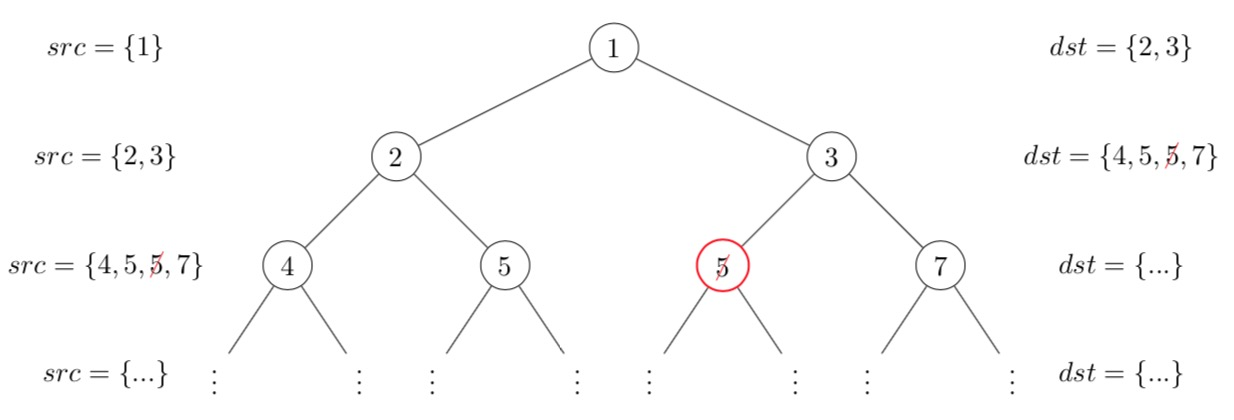
\includegraphics[width = \linewidth]{images/Distinct.jpg};
    \caption{Löschen von Duplikaten in einer Rekursionsstufe}
\end{figure}
Hierbei liegt der Knoten 5 so, dass er in der 2. Rekursionsstufe 2 Mal in der Auswahl auftaucht. DISTINCT entfernt das Duplikat. Die Ergebnismenge, entfernt um die
Duplikate, wird als Input für die nächste Rekursionsstufe verwendet.
Die Ausgabe des verschachtelten SELECT Statement sind die Nachbarn der Knoten, der angegebenen Rekursionstiefe. Wird zum Beispiel ein
verschachteltes SELECT Statement der Tiefe 3 erstellt, so gibt dieses Statement alle Nachbarn 3. Grades ausgehend vom Startknoten an. Der Nachteil bei dieser Methode ist, dass
Kreise in einem Graph nicht erkannt werden. Die Duplikatüberprüfung erfolgt nicht über mehrere Rekursionsstufen hinweg, sondern immer nur zwischen zwei Rekursionsstufen.
Der Ausführungsplan für ein verschachteltes SELECT der Tiefe 5 befindet sich im Anhang (siehe \ref{AusführungsplanCascadeSELECT}). Für die DISTINCT Überprüfung
wird auf jeder Rekursionsebene ein HashAggregate herangezogen. Die \textcolor{red}{Zugehörigkeitsüberprüfung} zur IN Klausel in der WHERE Bedingung ist in folgendem
Listing gegeben:
\begin{lstlisting}[language=SQL,caption = IN Klausel,frame=single, label={INKlauselFacebook} ]
    SELECT DISTINCT(dst) FROM relation_facebook WHERE src <@\textcolor{red}{IN}@> ()
\end{lstlisting}
Die Zugehörigkeitsüberprüfung erfolgt auf allen Rekursionsstufen, ausgenommen der ersten Rekursionsstufe, mit Hilfe eines \textcolor{red}{Hash Join}. Bevor der Hash Join
durchgeführt wird, wird zuerst der \textcolor{blue}{Hash} gebildet und anschließend ein \textcolor{orange}{Sequential Scan} durchgeführt:
\begin{lstlisting}[language=SQL,caption = Aufruf der DISTINCT Funktion,frame=single, label={WhereConditionCTE} ]
    ->  <@\textcolor{red}{Hash Join}@>  (cost=2713.40..4389.64 rows=88234 width=4) (actual time=11.821..17.797 rows=1709 loops=1)
    ->  <@\textcolor{orange}{Seq Scan}@> on relation_facebook relation_facebook_1  (cost=10000000000.00..10000001649.62 rows=100762 width=8) (actual time=0.004..4.822 rows=100762 loops=1)
    ->  <@\textcolor{blue}{Hash}@>  (cost=60.87..60.87 rows=19 width=4) (actual time=0.022..0.022 rows=4 loops=1)
\end{lstlisting}
Auf der ersten Rekursionsstufe erfolgt die Überprüfung der IN Klausel mit Hilfe eines \textcolor{red}{Index Scan}:
\begin{lstlisting}[language=SQL,caption = IndexScanFacebookRelation,frame=single, label={indexScanFacebookRelation} ]
    <@\textcolor{red}{Index Scan}@> using indexsrc on
    relation_facebook relation_facebook_4 (cost =0.29..44.00 rows =23 width =4) ( actual time =0.009..0.012 rows =27 loops =1)
    Index Cond: (src = 765)
\end{lstlisting}
Dieser wird nur auf der ersten Rekursionsstufe verwendet. Auf den tieferen Rekursionsstufen wird immer ein Sequential Scan vollzogen (vergleiche hierzu \ref{AusführungsplanCascadeSELECT} ). Der Grund dafür ist, dass nur auf der ersten Rekursionsstufe auf
einer Tabelle operiert wird auf der ein Index erstellt worden ist. In den tieferen Rekursionsstufen werden mit Hilfe der IN Klausel Zwischentabellen erstellt, auf denen kein Index existiert.
 Auf diesen Tabelle operiert das verschachtelte SELECT Statement jedoch die meiste Zeit, wesshalb die meiste Zeit ein sequential Scan verwendet wird.
\subsection{Graphtraversierung mit Hilfe von rekursiven INNER JOIN}
\label{postgresInnerJoin}
Bei der Graphtraversierung mit Hilfe von rekursiven INNER JOIN soll der Graph traversiert werden, indem die Relationentabelle immer wieder mit sich selber verknüpft wird.
Die Ausgabe ist, ähnlich wie bei der Graphtraversierung mit Hilfe von verschachteltem SELECT Statement, die Nachbarn der Knoten, die sich auf der mitgegebenen Rekursionsstiefe
befinden. Ein Beispielstatement für den rekursiven INNER JOIN ist im Anhang gegeben (siehe \ref{JOIN}). Der Ausführungsplan für die relation$\_$facebook Tabelle befindet sich
im Anhang (\ref{AusführungsplanINNERJOIN}). Fast alle Verknüpfungen werden mit Hilfe eines Hash Join vollzogen.Bei dem Ausführungsplan fällt der Merge Join auf, der sehr viel Zeit in Ansprich nimmt:
\begin{lstlisting}[language=SQL,caption = Merge JOIN,frame=single, label={mergeJoin} ]
    ->  Merge Join  (cost=89342.23..356052.39 rows=17747686 width=4) (actual time=112.509..1178.121 rows=8863706 loops=1)
\end{lstlisting}

\subsection{Graphtraversierung mit Hilfe von selbstgeschriebenen Stored Procedure}
\label{postgresRecursiveFunction}
Bei der Graphtraversierung mit Hilfe von selbstgeschriebenen Stored Procedure wird der Graph mit Hilfe eines selbst erstellten Stored Procedure, das sich selber bis
zu einer mit gegebenen Rekursionstiefe wieder aufruft, traversiert (siehe \ref{recursiveFunction}). Die \textcolor{red}{Abbruchbedingung} wird dem Stored Procedure in Form einer
Rekursionsstiefe mitgegeben.
\begin{lstlisting}[language=SQL,caption = Abbruchbedingung recursiveSearch,frame=single, label={AbbruchbedingungRecursiveSearch} ]
    CREATE OR REPLACE FUNCTION recursivesearch(tInput integer[], <@\textcolor{red}{iRecursionDepth integer} @>, sTable text) RETURNS SETOF integer AS
\end{lstlisting}
In jeder Rekursionsstufe erstellt das Script 2 temporäre Tabelle. Eine \textcolor{blue}{temporäre Tabelle} \footnote{Zuerst wurde das Script mit Hilfe einer standard Tabelle
erstellt. Dadurch war das Stored Procedure jedoch um den Faktor 7 langsamer. Es ist die Vermutung, dass durch die Anlage als temporäre Tabelle, die Tabelle im Shared Memory angelegt wird.
Hierdurch wird der Performancegewinn erzielt  \cite[S.26]{froehlich01})}
wird auf Basis eines \textcolor{red}{Eingabeparameter} (Datenstruktur Array) mit Hilfe des \textcolor{orange}{unnest Operator} erstellt.
\begin{lstlisting}[language=SQL,caption = Signatur recursiveSearch,frame=single, label={AbbruchbedingungRecursiveSearch} ]
    <@\textcolor{blue}{CREATE TEMPORARY TABLE} @> intermDst AS SELECT * FROM <@\textcolor{orange} {unnest} @> <@\textcolor{red}{(tInput)}@>;
\end{lstlisting}
Diese temporäre Tabelle besitzt eine Spalte. Diese Tabelle stellt die Spalte src der aktuellen Rekursionsstufe dar. Sie wird im \textcolor{red}{IN} Operator der WHERE Klausel verwendet
um die \textcolor{blue}{2. temporäre Tabelle} zu erstellen.
\begin{lstlisting}[language=SQL,caption = Erstellen 2. temporäre Tabelle,frame=single, label={AbbruchbedingungRecursiveSearch} ]
<@\textcolor{blue}{EXECUTE 'CREATE TEMPORARY TABLE} @> intermDst1 AS SELECT DISTINCT(dst) FROM ' || sTable || '
WHERE src <@\textcolor{red} {IN (SELECT * FROM intermDst)}'@>;
\end{lstlisting}
Die \textcolor{blue}{2. temporäre Tabelle} beinhaltet die Spalte dst der aktuellen Rekursionsstufe. Sie wird in ein \textcolor{red}{Array}
 umgewandelt
\begin{lstlisting}[language=SQL,caption = Erstellen des Aufrufarray,frame=single, label={AbbruchbedingungRecursiveSearch} ]
intermDst_ := <@\textcolor{red}{ARRAY}@>(SELECT * FROM <@\textcolor{blue}{intermDst1}@>);
\end{lstlisting}
intermDst\_ wird als \textcolor{red}{Aufrufparameter} für die nächste Rekursionsstufe mitgegeben. Darüber hinaus wird die nächst \textcolor{purple}{niedrigere Rekursionsstufe} und die
\textcolor{blue}{Tabelle} als Aufrufparameter an die \textcolor{orange}{Funktion} übergeben:
\begin{lstlisting}[language=SQL,caption = Aufrufen der nächst tieferen Rekursionsstufe,frame=single, label={AbbruchbedingungRecursiveSearch} ]
return query SELECT * FROM <@\textcolor{orange}{recursivesearch}@>(<@\textcolor{red}{intermDst\_}@>, <@\textcolor{purple}{iRecursionDepth - 1}@>, <@\textcolor{blue}{sTable}@>);
\end{lstlisting}
In der nächst tieferen Rekursionsstufe dient die 2. temporäre Tabelle als die Tabelle, die alle
src Spalten der aktuellen Rekursionsstufe beinhaltet. Die 2. temporäre Tabelle wird mit Hilfe von dynamischen \ac{SQL} \footnote{"Dynamisches SQL wird gerne verwendet,
da zur Zeit der Erstellung des Programms häufig nicht alle Parameter bekannt sind. Die Vervollständigung wird auf den Ausführungszeitpunkt verlagert. Darüber hinaus
ist es möglich, Programme zu erstellen, die in gewisser Weise generisch oder allgemeingültig sind."\cite[S.316 - 317]{froehlich01}} erstellt.
%\lstsetsql

%\end{figure}
%\subsection{Beurteilung}